% =============================================================
%  VVSC_Chuang_ChengShun_HW2.tex
%  AOE/CS/ME 6444 — Verification and Validation in Scientific Computing
%  Homework #2 — Application Description
%  Spring 2026 | Dr. Chris Roy
%  Authors: Jason Cusati & Cheng-Shun Chuang
% =============================================================
\documentclass[11pt,letterpaper]{article}

\usepackage[margin=1in,headheight=14pt]{geometry}
\usepackage{amsmath,amssymb}
\usepackage{booktabs}
\usepackage{graphicx}
\usepackage{xcolor}
\usepackage{hyperref}
\usepackage{caption}
\usepackage{subcaption}
\usepackage{array}
\usepackage{parskip}
\usepackage{float}
\usepackage{enumitem}
\usepackage{fancyhdr}
\usepackage{tikz}
\usetikzlibrary{arrows.meta, decorations.pathmorphing, patterns}

\hypersetup{colorlinks=true, linkcolor=blue, citecolor=blue, urlcolor=blue}

\pagestyle{fancy}
\fancyhf{}
\rhead{AOE/CS/ME 6444 — HW\,2}
\lhead{Cusati \& Chuang}
\cfoot{\thepage}

\newcolumntype{R}[1]{>{\raggedleft\arraybackslash}p{#1}}
\newcommand{\EI}{EI}

% =============================================================
\begin{document}

\begin{center}
  {\LARGE\bfseries Homework \#2: Application Description}\\[6pt]
  {\large AOE/CS/ME 6444 — Verification and Validation in Scientific Computing}\\
  {\large Spring 2026 \quad|\quad Instructor: Dr.\ Chris Roy}\\[4pt]
  {\large Jason Cusati \quad\&\quad Cheng-Shun Chuang}\\[2pt]
  {\normalsize Due: Thursday, February 26, 2026}
\end{center}
\vspace{6pt}
\hrule
\vspace{10pt}

% =============================================================
\section{Application Area}
\label{sec:app}

\textbf{Team:} Jason Cusati \& Cheng-Shun Chuang (2-person team).

\textbf{Application:} Structural assessment of a simply-supported residential wood header
under uniform distributed load using a finite-difference Euler--Bernoulli (EB) beam solver.

This application is directly relevant to residential construction engineering.
A \emph{header} (also called a lintel) is a horizontal structural member that spans a
door or window opening and carries the load of the framing above.
The ability to quickly and accurately size headers using a verified numerical solver forms
the backbone of an AI-assisted construction takeoff and design-check system being
developed as part of a broader research project.

% =============================================================
\section{System, Surroundings, and Environments}
\label{sec:system}

\subsection{Physical System}

The \textbf{system of interest} is a single horizontal beam spanning an opening
in a residential wood-framed wall.
A representative \emph{8-ft LVL (Laminated Veneer Lumber) header} is used as the
primary case study.
Table~\ref{tab:params} summarises the deterministic design parameters.

\begin{table}[ht]
\centering
\caption{Baseline system parameters for the 8-ft LVL residential header.}
\label{tab:params}
\begin{tabular}{llll}
  \toprule
  Parameter & Symbol & Value & Units \\
  \midrule
  Span                & $L$      & 96.0       & in  \\
  Cross-section width & $b$      & 3.5        & in  \\
  Cross-section depth & $d$      & 11.25      & in  \\
  Elastic modulus     & $E$      & 1,600,000  & psi \\
  Uniform load        & $q_0$    & 500        & lb/ft \\
  Moment of inertia   & $I = bd^3/12$ & 415.28 & in$^4$ \\
  Flexural rigidity   & $\EI$    & $6.645\times10^8$ & lb$\cdot$in$^2$ \\
  Allowable bending   & $F_b$    & 900        & psi \\
  Allowable shear     & $F_v$    & 180        & psi \\
  \bottomrule
\end{tabular}
\end{table}

\subsection{System Sketch}

Figure~\ref{fig:sketch} shows the simply-supported beam with uniform distributed
load and the key physical quantities.

\begin{figure}[ht]
  \centering
  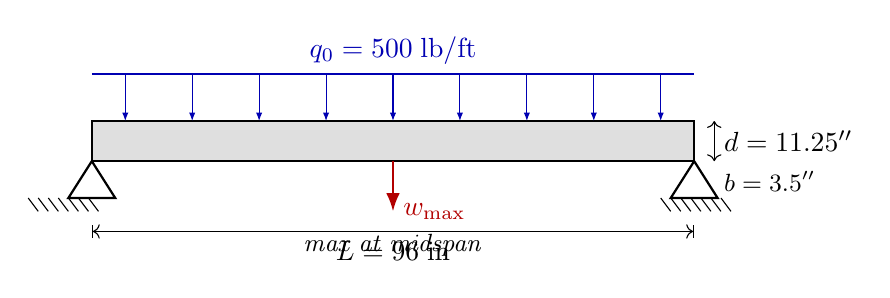
\begin{tikzpicture}[scale=0.85]
    % Beam body
    \fill[gray!25] (0,-0.3) rectangle (9,0.3);
    \draw[thick] (0,-0.3) rectangle (9,0.3);
    % UDL arrows
    \foreach \x in {0.5,1.5,...,8.5} {
      \draw[-{Latex[length=3pt]}, blue!70!black] (\x, 1.0) -- (\x, 0.3);
    }
    \draw[thick, blue!70!black] (0, 1.0) -- (9, 1.0);
    \node[blue!70!black] at (4.5, 1.35) {$q_0 = 500\;\text{lb/ft}$};
    % Supports
    \draw[thick] (0,-0.3) -- (-0.35,-0.85) -- (0.35,-0.85) -- cycle;  % pin
    \draw[thick] (9,-0.3) -- (8.65,-0.85) -- (9.35,-0.85) -- cycle;   % roller
    \foreach \x in {-0.45,-0.3,...,0.45} \draw (-0.45+\x-0.05,-0.85)--(-0.45+\x+0.1,-1.05);
    \foreach \x in {8.55,8.7,...,9.45} \draw (\x-0.05,-0.85)--(\x+0.1,-1.05);
    % Span annotation
    \draw[|<->|] (0,-1.35) -- (9,-1.35) node[midway,below] {$L = 96\;\text{in}$};
    % Cross-section annotation
    \draw[<->] (9.3,-0.3) -- (9.3,0.3) node[midway,right] {$d=11.25''$};
    \node[right] at (9.3,-0.6) {\small $b=3.5''$};
    % w_max arrow
    \draw[-{Latex}, red!70!black, thick] (4.5,-0.3) -- (4.5,-1.05)
      node[right,red!70!black] {$w_{\max}$};
    \node at (4.5,-1.55) {\small \textit{max at midspan}};
  \end{tikzpicture}
  \caption{Simply-supported LVL header under uniform distributed load.
    Pin support at $x=0$; roller support at $x=L$.
    Peak deflection $w_{\max}$ occurs at mid-span $x=L/2$.}
  \label{fig:sketch}
\end{figure}

\subsection{Surroundings and Environment}

The \textbf{surroundings} include:
\begin{itemize}[nosep]
  \item The roof framing assembly above the header (source of the applied load~$q_0$).
  \item The stud walls and jack studs at each end (providing the pinned/roller support
        reactions).
  \item The environmental conditions: standard interior temperature range
        (40--90\,°F), which has a minor effect on wood stiffness and is treated
        as a deterministic parameter in the baseline model.
\end{itemize}

\textbf{Uncertain inputs} that will be carried forward to later homeworks:
\begin{enumerate}[nosep]
  \item \textit{Aleatory uncertainty:} Elastic modulus $E$ varies due to natural wood
        and manufacturing variability:
        $E \sim \mathcal{N}(\mu_E = 1{,}600{,}000\;\text{psi},\;\sigma_E =
        160{,}000\;\text{psi})$ ($\mathrm{CoV} = 10\%$).
  \item \textit{Epistemic uncertainty:} Applied load $q_0$ is not known precisely;
        it is represented as an interval
        $q_0 \in [400,\; 600]\;\text{lb/ft}$ ($\pm 20\%$ of nominal).
\end{enumerate}

% =============================================================
\section{Mathematical Model: Governing PDE}
\label{sec:pde}

\subsection{Strong Form (PDE)}

The beam deflection $w(x)$ (positive downward) satisfies the 4th-order
Euler--Bernoulli BVP on $(0,L)$:
\begin{equation}
  \EI\,w''''(x) = q_0, \quad x \in (0, L),
  \label{eq:bvp}
\end{equation}
with simply-supported boundary conditions (no deflection, no moment at either end):
\begin{equation}
  w(0) = w(L) = 0, \qquad w''(0) = w''(L) = 0.
  \label{eq:bcs}
\end{equation}

\subsection{Derived Quantities}

The bending moment and shear force fields follow from the deflection:
\begin{equation}
  M(x) = -\EI\, w''(x), \qquad V(x) = -\EI\, w'''(x).
\end{equation}
The peak bending stress and shear stress at any cross-section are:
\begin{equation}
  \sigma = \frac{M}{S}, \quad S = \frac{bd^2}{6},
  \qquad
  \tau = \frac{3V}{2A}, \quad A = bd.
\end{equation}

\subsection{Closed-Form (Exact) Solution}

For constant $q_0$ and simply-supported ends the exact solution is:
\begin{equation}
  w_{\mathrm{exact}}(x) = \frac{q_0}{24\,\EI}
    \bigl(x^4 - 2L x^3 + L^3 x\bigr),
  \label{eq:exact}
\end{equation}
giving the System Response Quantities (SRQs):
\begin{equation}
  w_{\max} = \frac{5 q_0 L^4}{384\,\EI},
  \qquad
  M_{\max} = \frac{q_0 L^2}{8},
  \qquad
  \sigma_{\max} = \frac{M_{\max}}{S}.
\end{equation}

For the baseline parameters:
\[
  w_{\max}^{\mathrm{exact}} = 0.06935\;\text{in},\quad
  M_{\max}^{\mathrm{exact}} = 48{,}000\;\text{lb\cdot in},\quad
  \sigma_{\max}^{\mathrm{exact}} = 650.16\;\text{psi}.
\]

% =============================================================
\section{Numerical Method}
\label{sec:numerical}

\subsection{Finite-Difference Discretization}

Equation~\eqref{eq:bvp} is discretized on a uniform grid of $N$ equal intervals
(spacing $h = L/N$, nodes $x_i = ih$, $i = 0, \ldots, N$) using the standard
5-point central-difference stencil for $w''''$:
\begin{equation}
  \frac{\EI}{h^4}
  \bigl(w_{i-2} - 4w_{i-1} + 6w_i - 4w_{i+1} + w_{i+2}\bigr) = q_0,
  \quad i = 2, \ldots, N-2.
  \label{eq:stencil}
\end{equation}
The simply-supported conditions $w''(0)=w''(L)=0$ are enforced via
\emph{ghost-node elimination}: introducing virtual nodes $w_{-1}=-w_1$ and
$w_{N+1}=-w_{N-1}$ at the boundaries, the modified near-boundary rows become:
\begin{equation}
  \frac{\EI}{h^4}\bigl(5w_1 - 4w_2 + w_3\bigr) = q_0, \qquad
  \frac{\EI}{h^4}\bigl(w_{N-3} - 4w_{N-2} + 5w_{N-1}\bigr) = q_0.
\end{equation}

\subsection{Formal Order of Accuracy}

Taylor expansion of the 5-point stencil about node $x_i$ shows that all
derivative terms below order~4 cancel identically:
\begin{equation}
  w_{i-2} - 4w_{i-1} + 6w_i - 4w_{i+1} + w_{i+2}
  = h^4\,w_i'''' + \frac{h^6}{6}\,w_i^{(6)} + \mathcal{O}(h^8).
\end{equation}
Dividing by $h^4$ and using $\EI w'''' = q_0$ gives the local truncation error
$\tau_i = \frac{\EI h^2}{6} w_i^{(6)} + \mathcal{O}(h^4)$, confirming a
\textbf{formally second-order} ($p_{\mathrm{th}} = 2$) scheme.

\subsection{Linear System and Solver}

Assembling all $N+1$ equations yields the sparse symmetric positive-definite
system $K\mathbf{w} = \mathbf{q}$, where $K \in \mathbb{R}^{(N+1)\times(N+1)}$
is a pentadiagonal matrix with entries of order $\EI/h^4$.
This system is solved by dense LU factorisation (\texttt{numpy.linalg.solve}).
Since no iterative method is used, the \textbf{iterative error is identically zero}.

\subsection{Grid Strategy}

Five systematically-refined grids are employed (constant refinement ratio $r = 2$):

\begin{center}
\begin{tabular}{ccc}
  \toprule
  Level & $N$ & $h$ [in] \\
  \midrule
  1 (coarsest) & 10  & 9.600 \\
  2            & 20  & 4.800 \\
  3            & 40  & 2.400 \\
  4            & 80  & 1.200 \\
  5 (finest)   & 160 & 0.600 \\
  \bottomrule
\end{tabular}
\end{center}

The \textbf{parametric study grid} used for uncertainty propagation (HW4--HW5)
is $N = 20$ ($h = 4.800$~in), which balances numerical accuracy
($U_{\mathrm{NUM}} \approx 0.28\%$) with the computational throughput required
for 100s--1000s of LHS evaluations.

% =============================================================
\section{Planned VV\&UQ Sequence}
\label{sec:plan}

\begin{enumerate}
  \item \textbf{Code Verification (HW\,3):} Order-of-accuracy test against the
    exact solution~\eqref{eq:exact} on five systematically refined grids.
    Demonstrate $\hat{p} \approx 2$ for $w_{\max}$.
  \item \textbf{Solution Verification (HW\,4):} Richardson extrapolation and GCI
    analysis; round-off study (float32 vs.\ float64); $U_{\mathrm{NUM}}$ budget.
  \item \textbf{Model Validation (HW\,5):} Generate synthetic experimental data
    for $w_{\max}$ from $E = \mu_E \pm \sigma_E$; compute AVM and MAVM using
    Latin Hypercube Sampling over $E \sim \mathcal{N}(\mu_E, \sigma_E)$.
  \item \textbf{Predictive Uncertainty (Final Project):} Nested sampling (outer
    loop over $q_0 \in [400, 600]$~lb/ft, inner LHS over $E$); p-box
    generation; total uncertainty $=$ input UQ $+$ model form $+$ numerical.
\end{enumerate}

\end{document}
